% \documentclass{beamer}
% \usepackage{graphicx}
% \usepackage{multicol}
% \setlength{\columnseprule}{1pt}
%
% \graphicspath{{./fig/}}
% \usetheme{material}
% \input{embed_video.tex}
%
%% \newlength{\wdth}
%
%% \newcommand{\strike}[1]{\settowidth{\wdth}{#1}\rlap{\rule[.5ex]{\wdth}{.4pt}}#1}
%
%
%\begin{document}

% \input{embed_video}

\section{Applications}
% \topicFramePrimary{Applications}

\begin{frame}[label=app-110b]
\frametitle{When the real-time flow information is crucial?}
\begin{itemize}
	\item Time-varying on slow time scales (e.g. sediment transport)
    \item Unpredictable start and duration (biology) 
    \item Irreproducible or expensive % add suction feeding stuff, ceramic particle release stuff, rupture and breakage
	\item Control of the flow-dependent process, or control the flow % add wind turbine stuff
    \item Mobility required, field experiments, harsh environments
\end{itemize}
\end{frame}

\begin{frame}[label=app-0]{Applications}
\centering\cardImg{lab1}{\textwidth}
\end{frame}

\begin{frame}[label=app-112]{We can leave the lab}
\begin{multicols}{2}
    \cardImg{ldc3}{.49\textwidth}
    \cardImg{ldc_splitter}{.49\textwidth}
\end{multicols}
\end{frame}


\begin{frame}[label=iibr-4]{And now we are ready for the Environmental Wind Tunnel}
    \cardImg{wind_tunnel_photo_1}{0.9\textwidth}
\end{frame}
    
\begin{frame}[label=iibr-44]{We are ready for the Environmental Wind Tunnel}
  \centering\cardImg{ptv_wind_tunnel_photo1.png}{.9\textwidth}
\end{frame}
    
\begin{frame}[label=app-22]{We can use it on a rotation table}
    \embedvideo{\includegraphics[width=\textwidth]{fig/rotation.jpg}}{video/rotation.mp4}
\end{frame}
    
    
    \begin{frame}[label=app-111]{Microgravity space applications}   
    \begin{columns}
    \column{.3\textwidth}
        \cardImg{microgravity}{\linewidth}
    \column{.7\textwidth}
        \cardImg{space_3d_ptv}{\linewidth}
    \end{columns}
    \end{frame}
    
    \begin{frame}[label=app-2b]{Single camera with a four-view splitter}
    \centering\cardImg{kim/setup.png}{.95\textwidth}
    \end{frame}
    
    \begin{frame}[label=app-3b]{Four view splitter}
    \embedvideo{\includegraphics[width=\textwidth]{fig/kim/4views.png}}{fig/kim/Video1a.mp4}
    \end{frame}
    
    \begin{frame}[label=app-4b]{Turbulent jet flow}
        \centering\cardImg{kim/jet.png}{\textwidth}
    \end{frame}

    


\begin{frame}[label=app-81]{Single camera - multiple views}
    \centering\cardImg{ldc_splitter}{0.8\textwidth}
    \embedvideo{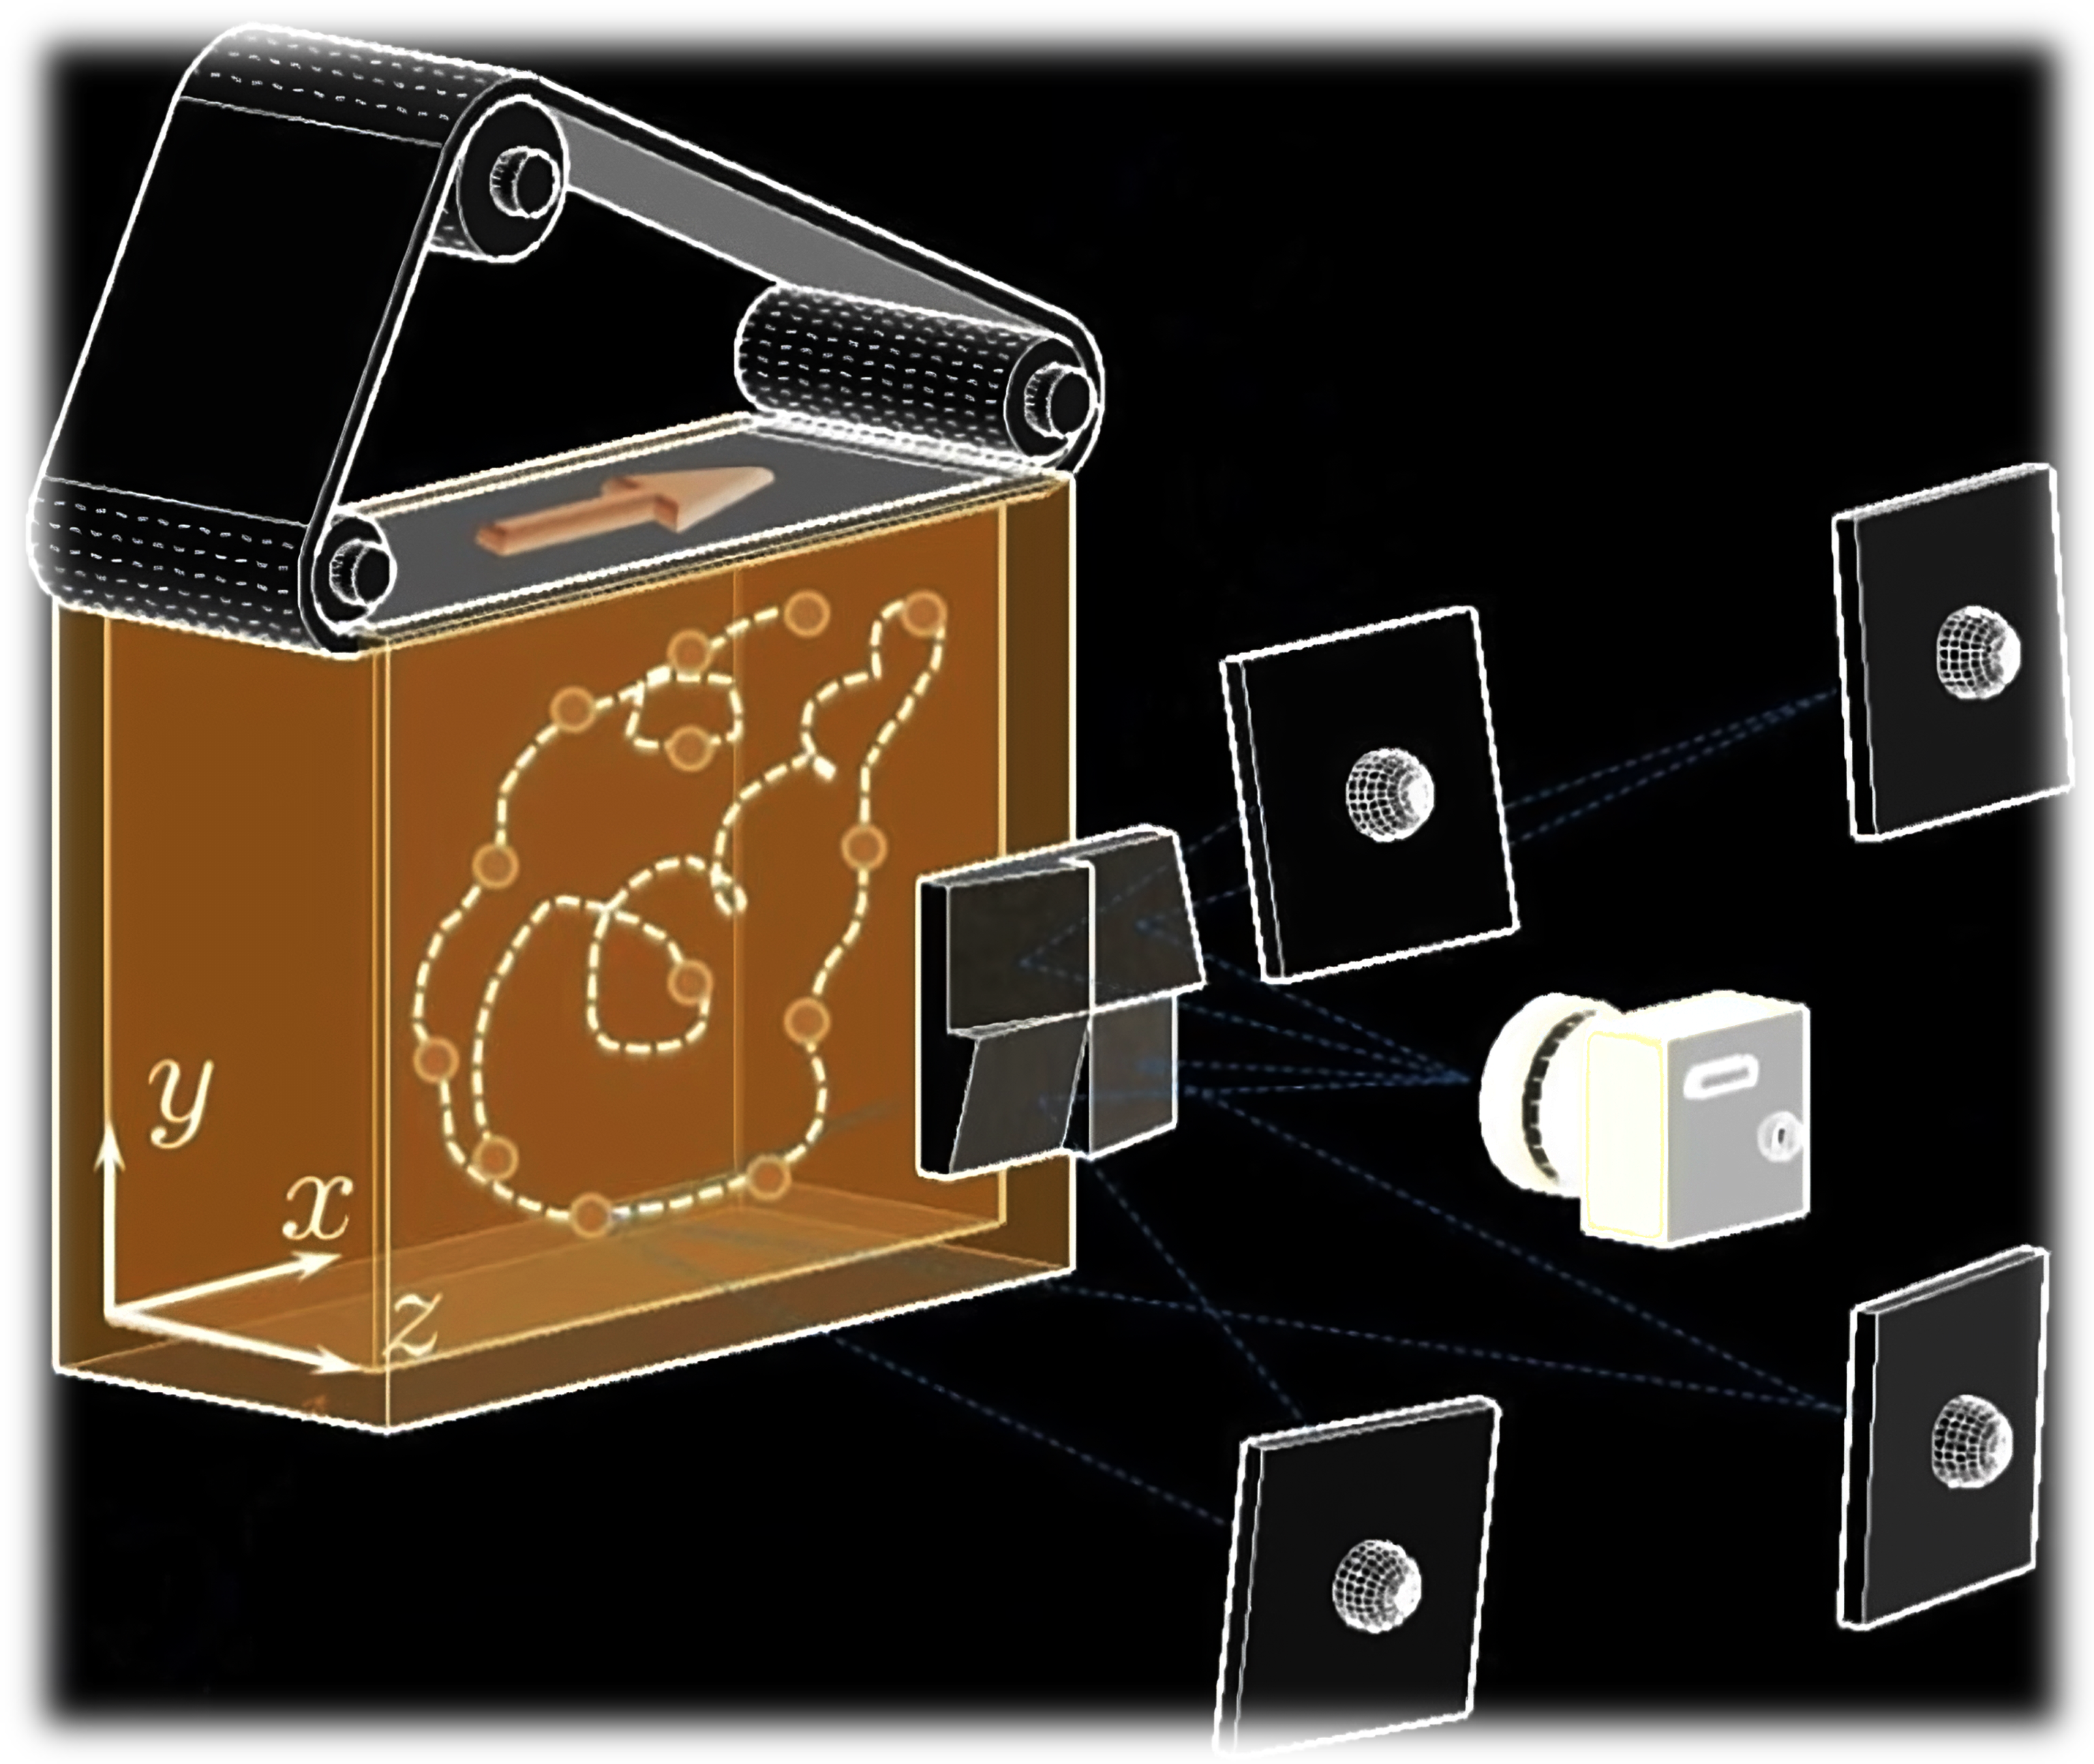
\includegraphics[width=\textwidth]{ldc_splitter}}{video/splitter_short.mp4}
    % \begin{cardTiny} A high speed camera with a four-view optical system \end{cardTiny}
    \end{frame}
    
    \begin{frame}[label=app-91]{3D-PTV can slide or rotate}
    \cardImg{sliding_ptv.jpg}{.9\textwidth}
    \begin{cardTiny} 
        Walpot et al. Meas. Sci. Tech. 2006. TU/e
    \end{cardTiny}
    \end{frame}
    

\begin{frame}[label=app-15]{MRI + 3D-PTV}
    \begin{columns}
    \column{.5\textwidth}
        \cardImg{mri2}{.35\textwidth}
        \cardImg{mri3}{.35\textwidth}
    \column{.5\textwidth}
        \centering\cardImg{mri1}{.5\textwidth}
    \end{columns}
\end{frame}

\begin{frame}[label=app-4a]{Aorta moving boundary + complex geometry, \href{https://www.dropbox.com/s/p1xnc7mefoqboti/aorta_rigid.mp4?dl=0}{ETH Zurich}}
\embedvideo{\includegraphics[width=\textwidth]{fig/aorta.png}}{video/aorta_rigid.mp4}
    \cardImg{aorta}{.9\textwidth}
\end{frame}
    
\begin{frame}[label=iibr-2]
    \begin{multicols}{2}
    \centering
    \cardImg{camera_system_laser.jpg}{0.49\textwidth}
    \cardImg{calibration_in_laser.jpg}{.49\textwidth}
    \end{multicols}
    \begin{cardTiny}
    Four cameras point into the measurement location, as seen from the test section inside the tunnel, and the calibration target is mounted on the traverse arm.
    \end{cardTiny}
\end{frame}
    
    %
\begin{frame}[label=iibr-1]
    \begin{multicols}{2}
    \centering\cardImg{img1.jpg}{.49\textwidth}
    \cardImg{camera_system_laser.jpg}{0.49\textwidth}
    \end{multicols}
\end{frame}
    
    % \begin{frame}{Pressurized air seeding devices}
    % \cardImg{seeding_sources_2.jpg}{0.9\textwidth}
    % \end{frame}
    
    % \begin{frame}{Seeding material}
    % \centering\cardImg{SiO2_003}{0.75\textwidth}
    % \end{frame}
    
    
    % \subsection{3D Particle Tracking Velocimetry}
    
    %\begin{frame}
    %\centering\cardImg{volumes.png}{.6\textwidth}
    %\begin{cardTiny}
    %Representation in the isometric view of the measurement sub-volumes within and above the canopy layer. The arrow points in the streamwise direction.
    %\end{cardTiny}
    %\end{frame}
    
    
    \begin{frame}[label=app-12]{Flow above the canopy}
    \centering
    \cardImg{flow_snapshot_above.jpg}{.9\textwidth}
    \end{frame}
    
    \begin{frame}[label=app-11]{Flow inside the canopy}
    \centering
    \cardImg{flow_snapshot_inside.jpg}{.9\textwidth}
    \end{frame}
    
    % \begin{frame}[label=app-10]{\href{./fig/flow_inside_laser.mp4}{Video clip}}
    % \centering\cardImg{flow_snapshot_inside.jpg}{\textwidth}
    % \end{frame}
    
%    
%    
    \begin{frame}[label=app-110a]{You could also do PIV on FPGA}
    \cardImg{real_time_piv_fpga.png}{\textwidth}
    \begin{cardTiny}
    Real-time particle image velocimetry based on FPGA technology, Munoz et al. IEEE (2009)
    \end{cardTiny}
    \end{frame}
%    
%    
\begin{frame}[label=app-11a]{Take it to the space - video credit: \href{https://www.dropbox.com/s/59ophf177gcfjzq/boiling_microgravity.mp4?raw=1}{ESA}}
    %\cardImg{maser_8}{0.3\textwidth}
    \embedvideo{\cardImg{space_3d_ptv}{0.8\textwidth}}{video/boiling_microgravity.mp4}
    \begin{cardTiny}
    Design and calibration of a four-headed camera for use in microgravity research, Willneff and Maas, ETH Zurich
    \end{cardTiny}
\end{frame}
    

\begin{frame}[label=app-1]
    \frametitle{Suction feeding events, courtesy of \href{https://www.dropbox.com/s/wcytdkxuxxvn4q0/fish_feeding.mp4?raw=1}{Prof. Roi Holzman, TAU}}
    \embedvideo{\includegraphics[width=\textwidth]{fig/fish_feeding.png}}{video/fish_feeding.mp4}
    %or this great video from Monterey Bay Aquarium 
    %
    %https://www.youtube.com/watch?v=umTqQSzKRmA    
\end{frame}
    
    \begin{frame}[label=app-2a]
    \frametitle{Flamingo underwater feeding - \href{https://www.dropbox.com/s/ic0l5npzon834l9/flamingo.mp4?raw=1}{San Diego Zoo}}
    % https://www.youtube.com/watch?v=-1BF2XqboOo
    \begin{center}
    \embedvideo{\includegraphics[width=\textwidth]{fig/flamingo.png}}{video/flamingo.mp4}
    \end{center}
    \end{frame}
    
    %
    
\begin{frame}[label=app-31]
    \frametitle{Colloids breakage events in turbulent flow, \href{https://www.dropbox.com/s/aufwfraotj5rll7/colloids1.mp4?raw=1}{ETH Zurich}}
    %https://pubs.acs.org/doi/10.1021/acs.langmuir.5b03804
    \embedvideo{\includegraphics[width=\textwidth]{fig/colloids1.png}}{video/colloids1.mp4}
\end{frame}
    
    %
    
\begin{frame}[label=app-3a]{Colloids breakage events in turbulent flow, \href{https://www.dropbox.com/s/8cimpwfsukf11u2/colloids2.mp4?raw=1}{ETH Zurich}}
    %https://pubs.acs.org/doi/10.1021/acs.langmuir.5b03804
    \embedvideo{\includegraphics[width=\textwidth]{colloid_sequence.jpg}}{video/colloids2.mp4}\end{frame}
    
    
\begin{frame}[label=app-5]{Real-time vortex identification for wind turbine blade pitch control - Caroline Braud}
    \begin{multicols*}{2}
    \cardImg{real_time_vortex_1}{.49\textwidth}
    \cardImg{real_time_vortex_2}{.49\textwidth}
    \end{multicols*}
\end{frame}
    
\begin{frame}[label=app-6]{Real-time sizing with 3D tracking - Rayne Ramirez, Uni. Oslo}
    \begin{multicols*}{2}
    \cardImg{drop-example}{.49\textwidth}
    \cardImg{drops}{.49\textwidth}
    \end{multicols*}
\end{frame}
    
\begin{frame}[label=app-7]{Fibers - \href{https://www.dropbox.com/s/y5gf55qqeyq5ljr/fibers.mp4?raw=1}{Stefano Brizzolara, ETH Zurich}}
    % https://twitter.com/stebrizzo94/status/1525577322144976910?s=20
    \embedvideo{\includegraphics[height=\textheight]{fibers.png}}{video/fibers.mp4}
\end{frame}

\begin{frame}[label=app-8a]{Microplastics in a vortex - \href{https://www.dropbox.com/s/in5ewv968dy9j3q/microplastics.mp4?raw=1}{Turbulence Structure Laboratory}}
    % Imaging‑based 3D particle tracking system forfield characterization ofparticle dynamics inatmospheric flows
    \embedvideo{\includegraphics[height=\textheight]{trajects.png}}{video/microplastics2.mp4}\\
    Bristow et al. Exp. Fluids, 2023
\end{frame}
    
\begin{frame}[label=app-8]{Drone vs turbulence - \href{https://www.dropbox.com/s/3lav5rf6s8su6f5/drone.mp4?raw=1}{University of Minnesota}}
    % Imaging‑based 3D particle tracking system forfield characterization ofparticle dynamics inatmospheric flows
    \embedvideo{\includegraphics[height=\textheight]{drone.png}}{video/drone.mp4}\\
    Bristow et al. Exp. Fluids, 2023
\end{frame}
    
\begin{frame}[label=app-9]{Soon we could do it using AR/VR}
    \cardImg{mr_ptv_photo}{0.8\textwidth}
    Chivers, T. Uni. Vermont, MSc Thesis, 2023
\end{frame}
    
    
\begin{frame}[label=app-811]{Turbulent flow inside an urban canopy model at \href{https://www.dropbox.com/s/9x43i2uk9q38fho/flow_inside_laser.mp4?raw=1}{IIBR wind tunnel}}
    \embedvideo{\includegraphics[width=\textwidth]{flow_snapshot_inside.jpg}}{video/flow_inside_laser.mp4}
\end{frame}
%    

%\end{document}